\documentclass[aspectratio=169,12pt]{beamer}
\usepackage{amsmath}
\usepackage{amssymb}
\usepackage[most]{tcolorbox}
\usepackage{tikz}
\usepackage{graphicx}
\usepackage[sfdefault,lf]{FiraSans}
\renewcommand{\familydefault}{\sfdefault}
\setlength{\parindent}{0pt}
\everymath{\displaystyle}

\setbeamertemplate{navigation symbols}{}
\setbeamertemplate{footline}{}
\setbeamertemplate{headline}{}

\definecolor{mmpageWhite}{HTML}{FCFBF7}
\definecolor{mmtanSoft}{HTML}{F7F5EF}
\definecolor{mmgreenDeep}{HTML}{244B2C}
\definecolor{mmgreenLeaf}{HTML}{5D8A56}
\definecolor{mmgreenSoft}{HTML}{E4EFD9}
\definecolor{mmtext}{HTML}{163221}

\setbeamercolor{background canvas}{bg=mmpageWhite}
\setbeamercolor{normal text}{fg=mmtext,bg=mmpageWhite}

\newtcolorbox{MMProblemCard}[1][]{enhanced,breakable=false,colback=white,colframe=black,boxrule=1.0pt,arc=5pt,left=3pt,right=3pt,top=2pt,bottom=2pt,before skip=0pt,after skip=0pt,height=0.26\textheight,valign=top,#1}
\newcommand{\KoruIcon}{\raisebox{-0.2em}{
\includegraphics[height=1.05em]{../../SITE/header-logo.png}}}
\newcommand{\HoeIcon}{\raisebox{-0.2em}{
\includegraphics[height=1.05em]{../../SITE/hoe.png}}}
\newcommand{\ScaffoldIcons}[1]{\ifcase#1\or \HoeIcon\or \HoeIcon\hspace{0.22em}\KoruIcon\or \KoruIcon\hspace{0.22em}\KoruIcon\hspace{0.22em}\KoruIcon\fi}
\newcommand{\WorksheetTitle}[2]{%
  {\colorbox{mmtanSoft}{\parbox[c][2.0em][c]{0.975\linewidth}{%
    \hspace{0.25em}{\Large\bfseries\textcolor{mmgreenDeep}{#1}\hfill\ScaffoldIcons{#2}}}}
  \par\vspace{0.08em}{\color{mmgreenLeaf}\rule{\linewidth}{2.0pt}}\par\vspace{0.04em}}
}
\newcommand{\MMProblem}[2]{\begin{MMProblemCard}\raggedright\small\textbf{#1.} #2\par\end{MMProblemCard}}

\setbeamertemplate{background}{
 \begin{tikzpicture}[remember picture,overlay]
 \draw[black,line width=1.5pt,rounded corners=10pt]
 ([xshift=0.45cm,yshift=-0.45cm]current page.north west)
 rectangle
 ([xshift=-0.45cm,yshift=0.45cm]current page.south east);
 \end{tikzpicture}
}

% Default worksheet generation rules:
% use notes-style beamer pages
% use bordered cards for individual problems
% target 9 problems per frame in a 3x3 grid
% target 3 frames per scaffold by default where content allows

\begin{document}\begin{frame}[t]
\WorksheetTitle{Push Tasks}
\vspace{-0.18em}
\begin{columns}[T,onlytextwidth]
\begin{column}{0.32\textwidth}\MMProblem{1}{Find the perimeter.\\[0.4em]
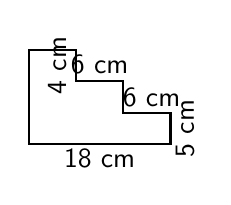
\begin{tikzpicture}[x=0.20cm,y=0.20cm,baseline=(current bounding box.center)]
  \draw[thick] (0,0)--(9,0)--(9,2)--(6,2)--(6,4)--(3,4)--(3,6)--(0,6)--cycle;
  \node at (4.5,-0.9) {18 cm};
  \node[rotate=90] at (9.9,1) {5 cm};
  \node at (7.8,3.0) {6 cm};
  \node at (4.5,5.1) {6 cm};
  \node[rotate=90] at (1.8,5) {4 cm};
\end{tikzpicture}}\end{column}
\begin{column}{0.32\textwidth}\MMProblem{2}{Find the perimeter.\\[0.4em]
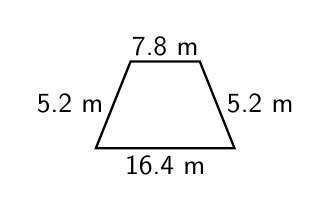
\begin{tikzpicture}[x=0.22cm,y=0.22cm,baseline=(current bounding box.center)]
  \draw[thick] (0,0)--(8,0)--(6,5)--(2,5)--cycle;
  \node at (4,-1.0) {16.4 m};
  \node at (4,5.9) {7.8 m};
  \node at (1.0,2.6) [left] {5.2 m};
  \node at (7.0,2.6) [right] {5.2 m};
\end{tikzpicture}}\end{column}
\begin{column}{0.32\textwidth}\MMProblem{3}{Find the perimeter.\\[0.4em]
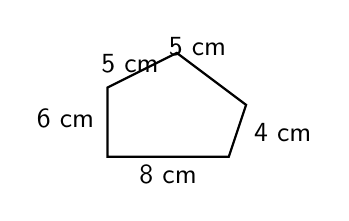
\begin{tikzpicture}[x=0.22cm,y=0.22cm,baseline=(current bounding box.center)]
  \draw[thick] (0,0)--(7,0)--(8,3)--(4,6)--(0,4)--cycle;
  \node at (3.5,-1.0) {8 cm};
  \node at (7.9,1.4) [right] {4 cm};
  \node at (5.2,6.4) {5 cm};
  \node at (-0.2,2.2) [left] {6 cm};
  \node at (1.3,5.4) {5 cm};
\end{tikzpicture}}\end{column}
\end{columns}
\vspace{0.45em}
\begin{columns}[T,onlytextwidth]
\begin{column}{0.32\textwidth}\MMProblem{4}{Find the perimeter.\\[0.4em]
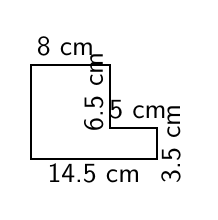
\begin{tikzpicture}[x=0.20cm,y=0.20cm,baseline=(current bounding box.center)]
  \draw[thick] (0,0)--(8,0)--(8,2)--(5,2)--(5,6)--(0,6)--cycle;
  \node at (4,-0.9) {14.5 cm};
  \node[rotate=90] at (8.9,1) {3.5 cm};
  \node at (6.8,3.2) {5 cm};
  \node[rotate=90] at (4.0,4.3) {6.5 cm};
  \node at (2.2,7.2) {8 cm};
\end{tikzpicture}}\end{column}
\begin{column}{0.32\textwidth}\MMProblem{5}{The perimeter of a rectangle is 52 cm. Its length is 4 cm more than its width. Find both dimensions.}\end{column}
\begin{column}{0.32\textwidth}\MMProblem{6}{An isosceles triangle has perimeter 31 cm. The equal sides are 9 cm each. Find the third side.}\end{column}
\end{columns}
\vspace{0.45em}
\begin{columns}[T,onlytextwidth]
\begin{column}{0.32\textwidth}\MMProblem{7}{A square and a rectangle both have perimeter 24 cm. The square has side 6 cm. Give one possible pair of whole-number dimensions for the rectangle that is not a square.}\end{column}
\begin{column}{0.32\textwidth}\MMProblem{8}{Maia walks once around a field shaped like a trapezium with sides 42 m, 35 m, 28 m and 35 m. How far does she walk in 3 laps?}\end{column}
\begin{column}{0.32\textwidth}\MMProblem{9}{A rectangle is widened by 3 cm and its perimeter increases by 6 cm. Explain why this always happens.}\end{column}
\end{columns}
\end{frame}
\begin{frame}[t]
\WorksheetTitle{Push Tasks}
\vspace{-0.18em}
\begin{columns}[T,onlytextwidth]
\begin{column}{0.32\textwidth}\MMProblem{1}{Which has the greater perimeter: a \mbox{$7$} cm by \mbox{$11$} cm rectangle or a triangle with sides \mbox{$8$} cm, \mbox{$9$} cm and \mbox{$12$} cm? How much greater?}\end{column}
\begin{column}{0.32\textwidth}\MMProblem{2}{A regular pentagon has perimeter 47.5 cm. Find one side length.}\end{column}
\begin{column}{0.32\textwidth}\MMProblem{3}{A builder used \mbox{$36$} m of timber around the edge of a rectangular deck. If the width is \mbox{$7$} m, find the length.}\end{column}
\end{columns}
\vspace{0.45em}
\begin{columns}[T,onlytextwidth]
\begin{column}{0.32\textwidth}\MMProblem{4}{}\end{column}
\begin{column}{0.32\textwidth}\MMProblem{5}{}\end{column}
\begin{column}{0.32\textwidth}\MMProblem{6}{}\end{column}
\end{columns}
\vspace{0.45em}
\begin{columns}[T,onlytextwidth]
\begin{column}{0.32\textwidth}\MMProblem{7}{}\end{column}
\begin{column}{0.32\textwidth}\MMProblem{8}{}\end{column}
\begin{column}{0.32\textwidth}\MMProblem{9}{}\end{column}
\end{columns}
\end{frame}
\end{document}
